\section{The Large Hadron Collider at CERN}%
\label{sec:lhc}

The LHC~\cite{Evans:2008zzb} is a circular proton and heavy-ion collider
experiment located at CERN\footnote{From the French \emph{Conseil Européen pour
    la Recherche Nucléaire} referring to both the research organisation and the
  location of the laboratory sites.} at the French--Swiss border in Geneva,
Switzerland. At present, the LHC is the world's highest-energy, laboratory-based
particle collider experiment with proton beam energies of up to \SI{6.8}{\TeV}
and proton--proton (\pp) centre-of-mass energies, $\sqrt{s}$, of up to
\SI{13.6}{\TeV}. The focus of this section lies on the operation of the LHC
using beams of protons.

The LHC was constructed in the former tunnel of the CERN Large Electron-Positron
Collider (LEP) with a circumference of \SI{26.7}{\kilo\metre}, first becoming
operational in 2008. It is a synchrotron consisting of two counter-rotating
beams of protons that are accelerated using alternating electric fields in
superconducting radio frequency resonators/cavities. The beams are bent into a
cyclic trajectory around the LHC ring using superconducting dipole magnets with
field strengths of about \SI{8}{\tesla}. Along the ring, numerous quadrupole
magnets are used for controlled focusing and defocusing of the proton beams.
% Synchrotron: 1232 dipoles (superconducting) -> Magnetic field of
% \SI{8.3}{\tesla} required for \SI{7}{\TeV} beam energy operation
The proton beams consist of localised packages of ca.\ $10^{11}$ protons,
herafter referred to as bunches, circulating in the LHC with a minimum spacing
in time of \SI{25}{\nano\second}~\cite{Evans:2008zzb}.

To reach proton energies necessary for the injection into the LHC, the
infrastructure of the CERN accelerator complex is used, which is schematically
depicted in~\Cref{fig:cern_accelerator_complex}. Protons are first accelerated
in LINAC 2\footnote{Short for \textbf{lin}ear \textbf{ac}celerator.}, the Proton
Synchrotron Booster (BOOSTER), the Proton Synchrotron (PS), and finally in the
Super Proton Synchrotron (SPS) after which the beams are injected into the LHC
with proton energies of \SI{450}{\GeV}~\cite{Evans:2008zzb}. The protons are
further accelerated in the LHC until the target energy is reached. At this
point, the beams are brought into collision at four points, the interaction
points (IPs), along the ring. Four large experiments are situated at these IPs
to observe and record particle collision events at the LHC:
ATLAS~\cite{PERF-2007-01}, CMS~\cite{CMS-CMS-00-001},
ALICE~\cite{ALICE:2008ngc}, and LHCb~\cite{LHCb:2008vvz}. The ATLAS and CMS
experiments are particle detector experiments targeting largely overlapping,
extensive physics programmes, while the ALICE and LHCb are more specialised
experiments. The ALICE experiment studies the production of the quark-gluon
plasma, a state of matter with asymptotically free quarks and gluons occurring
at temperatures similar to those right after the Big Bang, in heavy-ion
collisions. The LHCb experiment investigates the nature the matter-antimatter
asymmetry in the universe by studying CP violation in decays of hadrons
containing $b$-quarks. Several smaller experiments are installed at the LHC to
study physics processes at small angles with respect to the beamline of the LHC
or exotic particles. These experiments are LHCf~\cite{LHCf:2008lfy},
TOTEM~\cite{TOTEM:2008lue}, and
MoEDAL~\cite{MoEDAL:2009jwa}.\footnote{FASER~\cite{FASER:2019aik} and SND\@LHC.}

\begin{figure}[htbp]
  \centering

  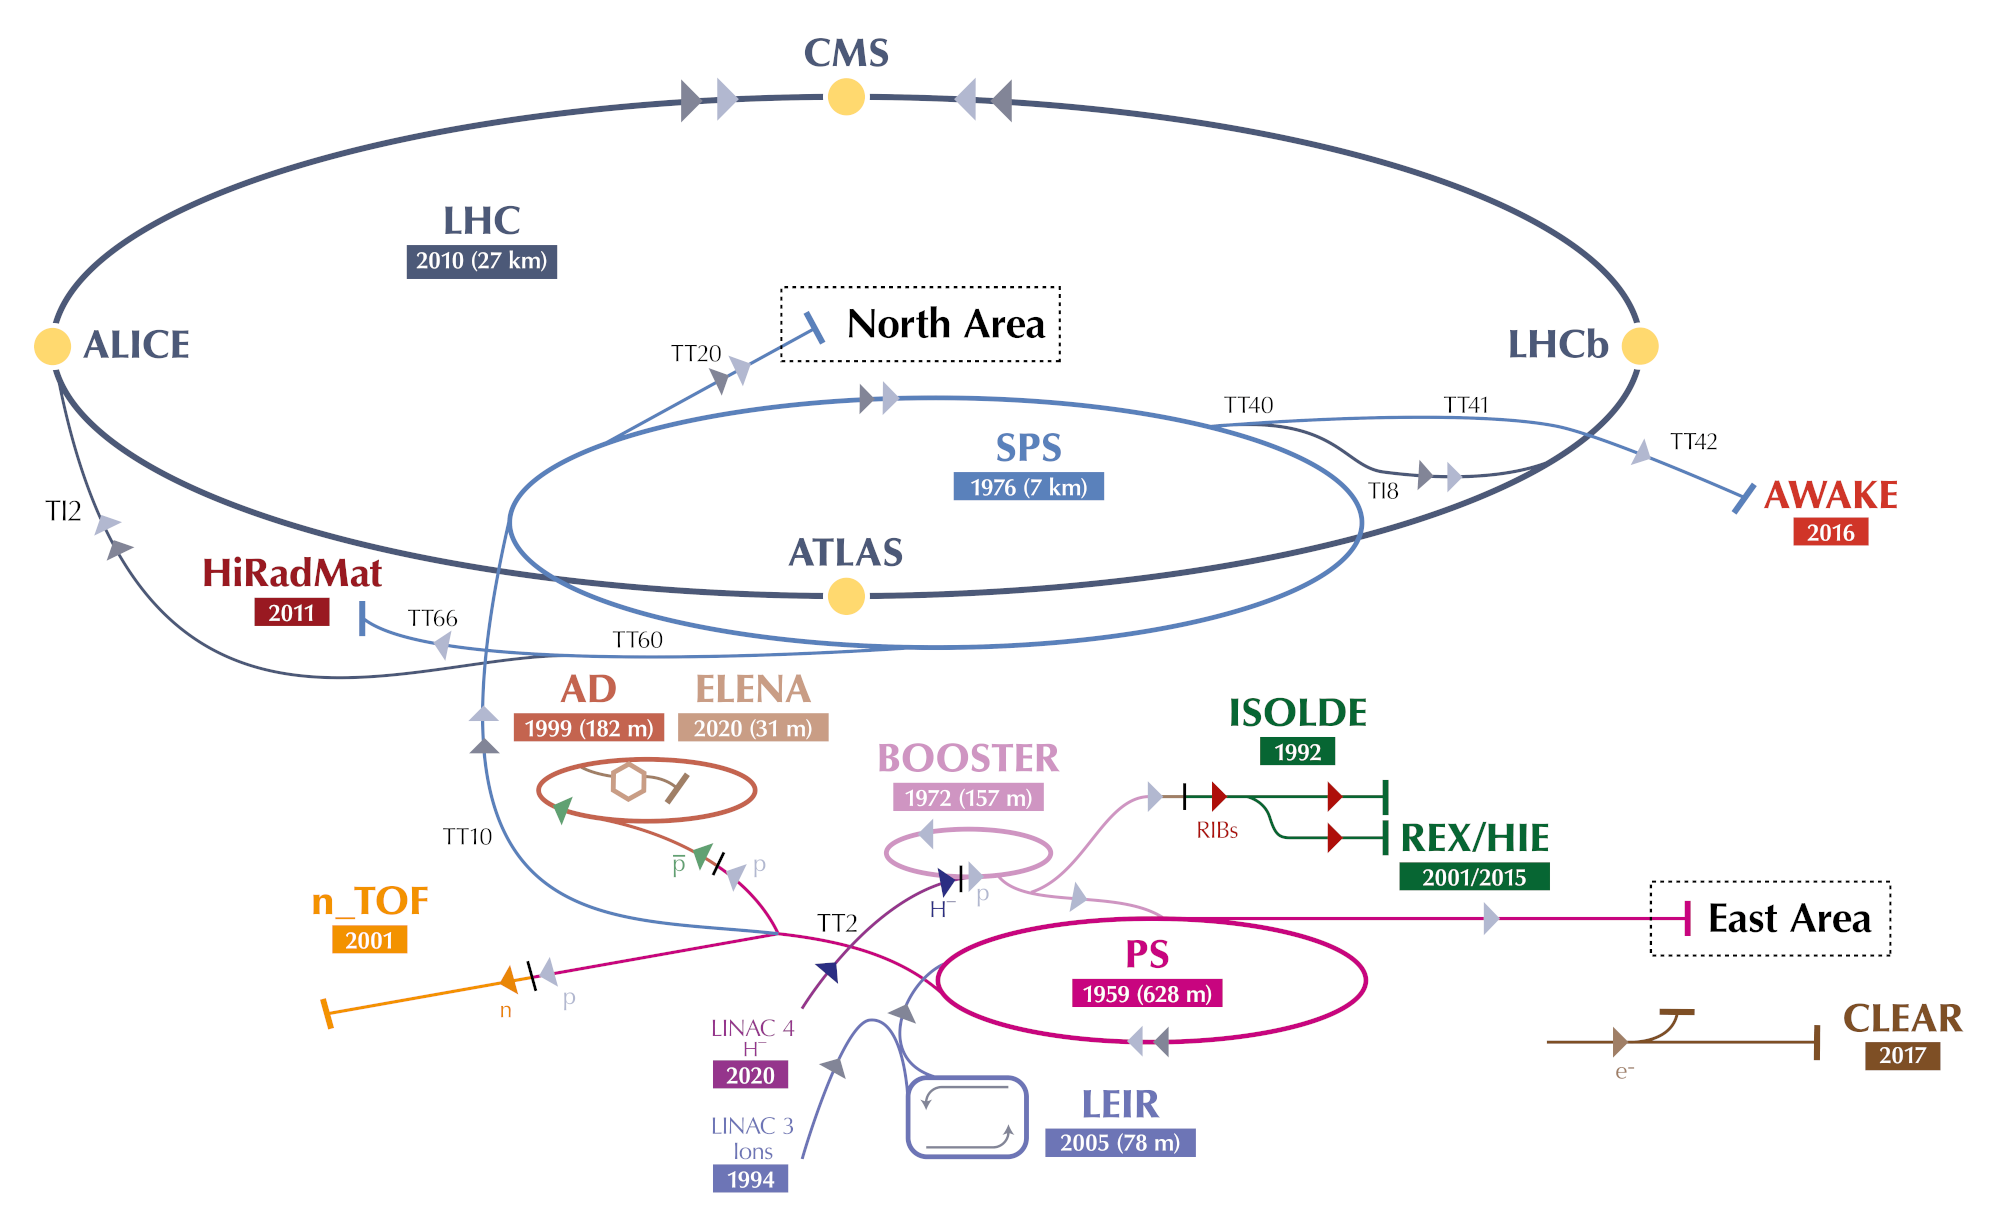
\includegraphics[width=0.9\textwidth, trim=10.5cm 44cm 2cm 20cm,
  clip]{lhc/cern_complex}

  \caption{The CERN accelerator complex in August 2018. The image is adapted
    from Ref.~\cite{Mobs:2684277}.}%
  \label{fig:cern_accelerator_complex}
\end{figure}

LHC operation for the main physics programmes of the experiments started in 2010
with \pp-collisions at $\sqrt{s} = \SI{7}{\TeV}$. In 2012, the centre-of-mass
energy was increased to \SI{8}{\TeV}. The data-taking period from 2010--2012 is
referred to as \emph{Run~1} of the LHC. After extensive upgrades of the LHC and
the detectors, the LHC restarted operation with \pp-collisions at
$\sqrt{s} = \SI{13}{\TeV}$ in \emph{Run~2} which took place from
2015--2018. After another shutdown of LHC and experiments, data-taking
recommenced in 2022 with Run~3, reaching unprecedented energy scales of
$\sqrt{s} = \SI{13.6}{\TeV}$. At present, Run~3 is forseen to last until the end
of 2025.

An important parameter of a particle collider is the instantaneous luminosity,
$L$, at a given IP as it directly relates the expected rate of collision events
from a process with its cross-section, $\sigma$, according to
\begin{align*}
  \frac{\mathrm{d}N}{\mathrm{d}t} = L \sigma \,\text{.}
\end{align*}
Consequently, the expected number of events observed over a time interval is
given by $N = L_{\text{int}} \, \sigma$, where
$L_{\text{int}} = \int \mathrm{d}t \, L(t)$ is the integrated
luminosity.\footnote{Assuming the cross-sections are time-independent.}



When searching for rare processes, it is generally desirable to achieve the
largest possible instantaneous luminosities .

However, difficulties arise in the form of inelastic \pp-collisions


The peak instantaneous luminosity at the IP of the ATLAS experiment ranged from
\SIrange{0.5}{1.9}{\per\centi\metre\squared\per\second} during Run~2 of the
LHC~\cite{ATLAS-CONF-2019-021}.


$\sigma_{\text{inelastic}}$ of \pp at $\sqrt{s} = \SI{13}{\TeV}$ is
\SI{80}{\milli\barn}~\cite{STDM-2015-05}

\Cref{fig:atlas_mu}

\Cref{fig:atlas_int_lumi_vs_time}


% Luminosity or pile-up plots?
% https://twiki.cern.ch/twiki/bin/view/AtlasPublic/LuminosityPublicResultsRun2

\begin{figure}[htbp]
  \centering

  \begin{subfigure}{0.47\textwidth}
    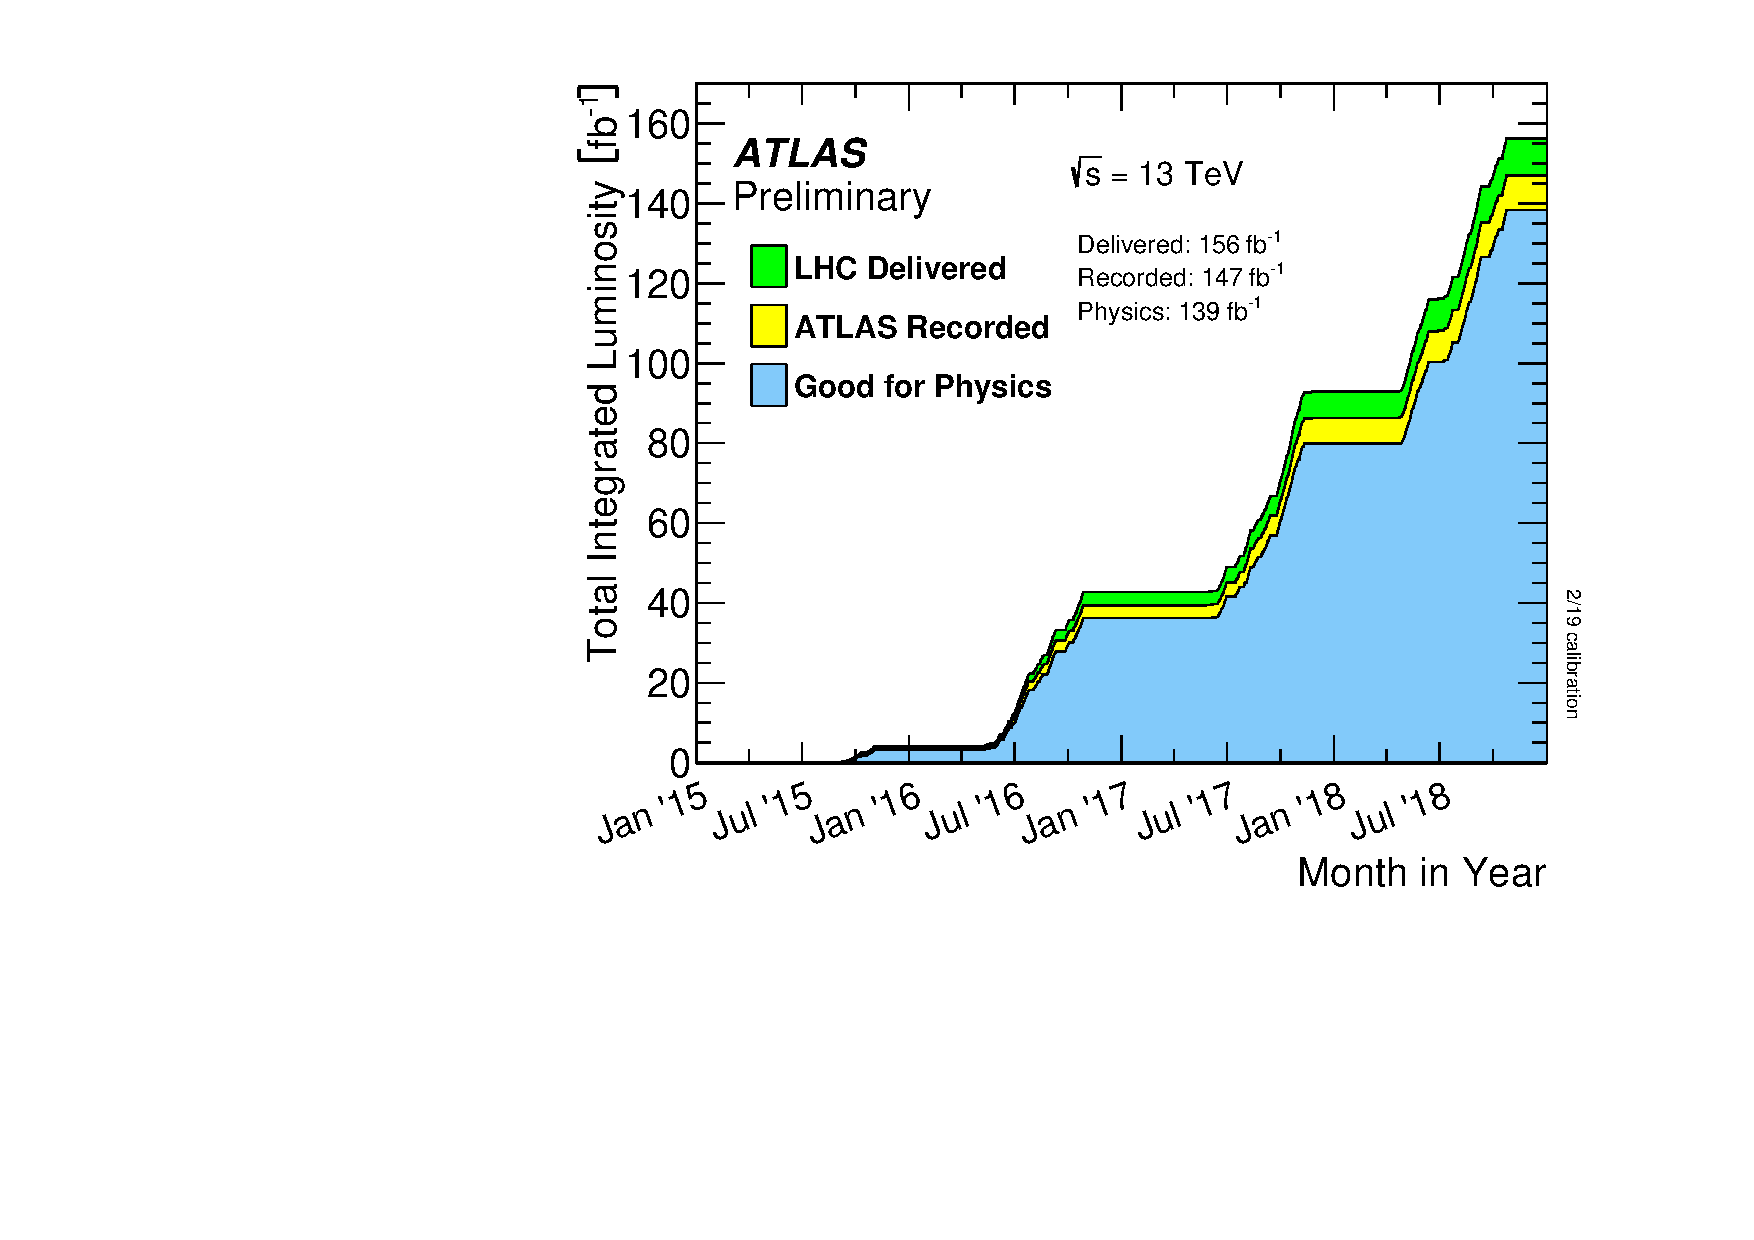
\includegraphics[width=\textwidth]{lhc/int_lumi_vs_time}
    \subcaption{}%
    \label{fig:atlas_int_lumi_vs_time}
  \end{subfigure}\hspace*{0.02\textwidth}%
  \begin{subfigure}{0.47\textwidth}
    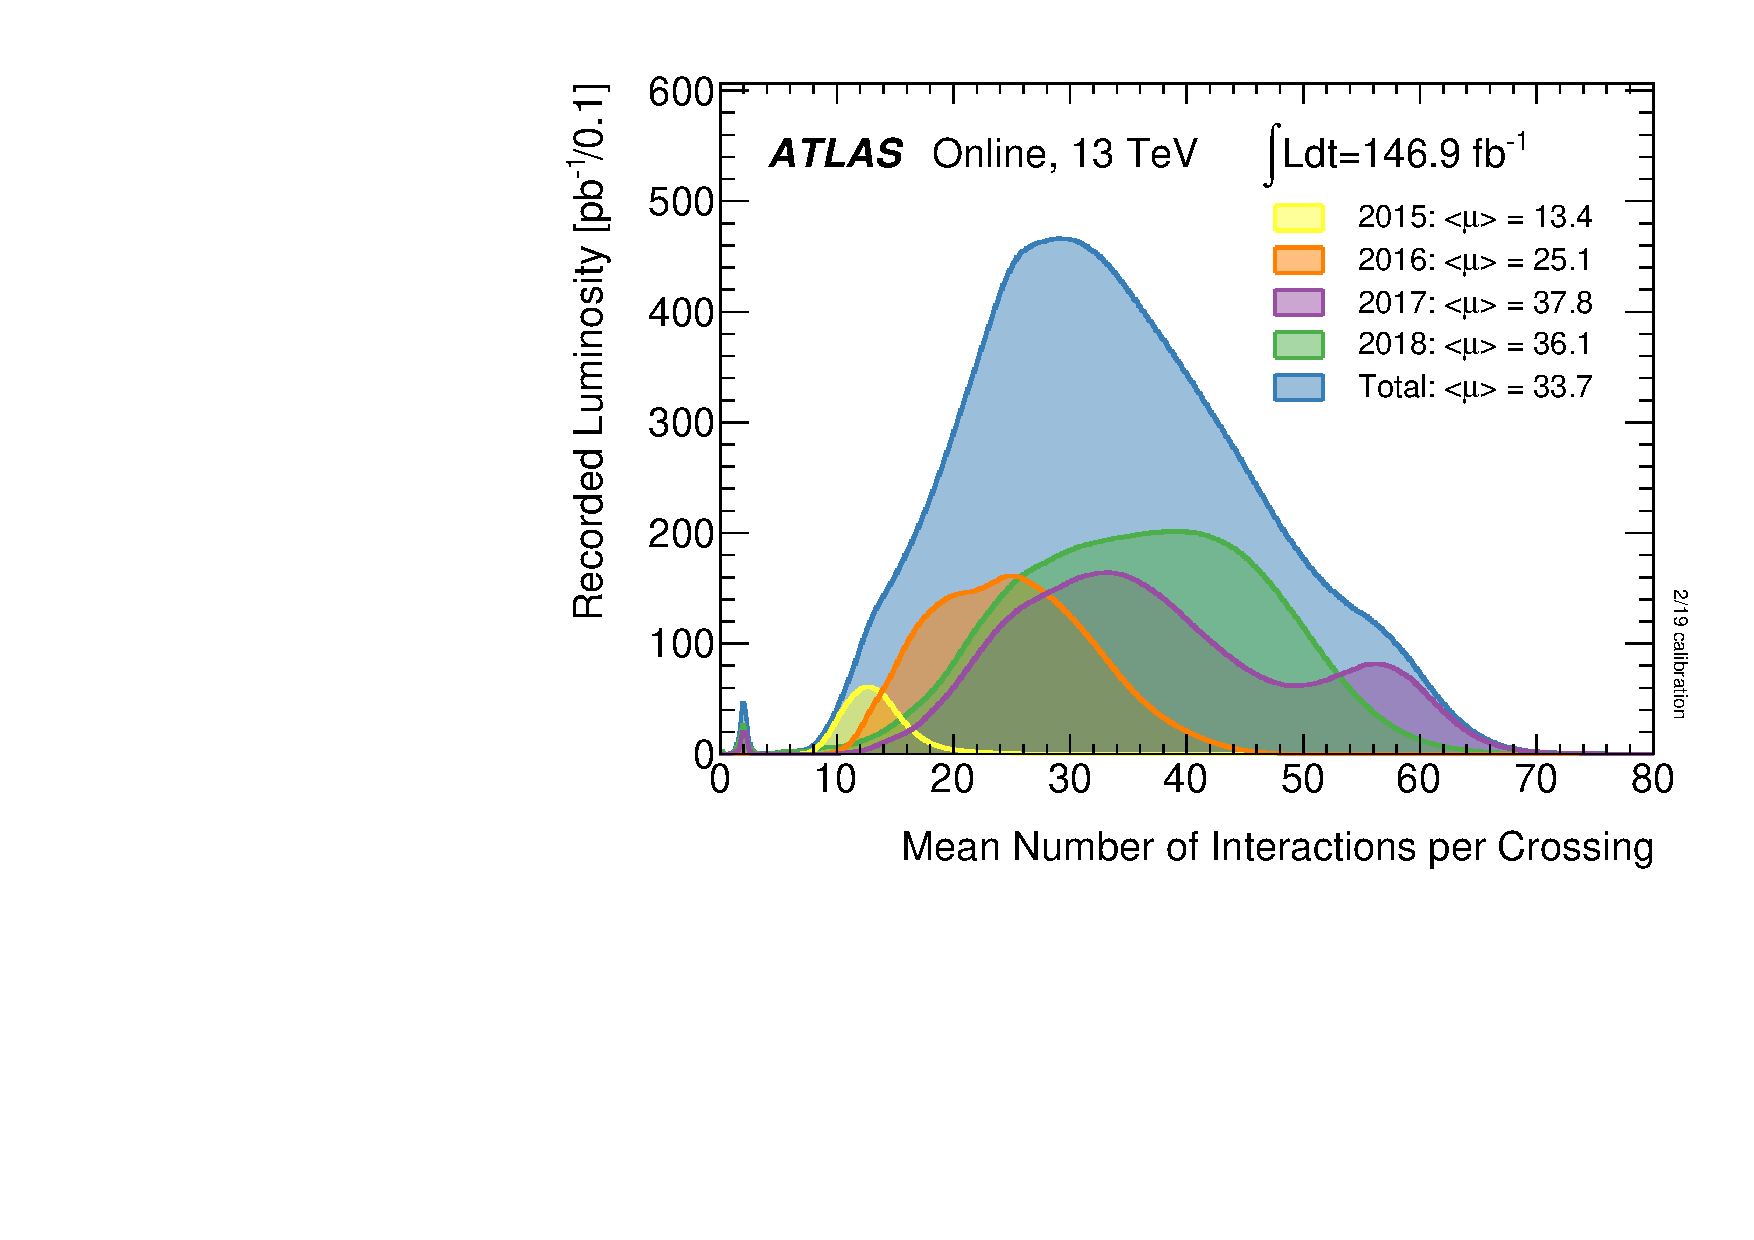
\includegraphics[width=\textwidth]{lhc/mu_2015_2018}
    \subcaption{}%
    \label{fig:atlas_mu}
  \end{subfigure}

  \caption{The integrated luminosity as a function of time (a) and the
    luminosity-weighted mean number of interactions per bunch-crossing (b) of
    the LHC in \pp operation mode during Run~2. In figure (a), the integrated
    luminosity delivered by the LHC (green), recorded by the ATLAS detector
    (yellow), and the integrated luminosity of the \pp-collision dataset passing
    the data-qualtiy criteria~\cite{DAPR-2018-01} of the ATLAS collaboration
    (blue) is shown. The mean number of interactions per bunch-crossing, $\mu$,
    is calculated from the instantaneous luminosity assuming an inelastic \pp
    cross-section at $\sqrt{s} = \SI{13}{\TeV}$ of \SI{80}{\milli\barn}. The
    figures are taken from~\cite{atlas_luminosity_summary_plots}.}%
  \label{fig:lumi_and_pu}
\end{figure}

% The physics programme of the LHC is planned to conclude by ca.\ 2040 after an
% upgrade ~\cite{hl_lhc}.
This thesis is mostly concerned with the \pp-collision during Run~2 of the LHC.


Centre-of-mass energy and instantaneous / integrated luminosity.

% - Energy to produce Higgs boson pairs can, at present, not be achieved with
%   electron positron colliders -> VHH production which would require CMS in excess of 300 GeV

% - Cross section of HH production - Ndot = L * sig
% - LHC proton and heavy-ion collider, though exclusively working with \pp
% collision data.

\begin{itemize}

\item What is the goal of the LHC? -> energy frontier (protons instead of
  electrons due to reduced synchrotron radiation)

\item Performance characteristics of the \pp operation of the LHC during Run~2:

  \begin{itemize}
  \item Bunches \& Bunch spacing: 2556 (\SI{25}{\nano\second}) -- but 2808 RF<
    buckets (not all filled)
  \item Luminosity: \SI{2.1e34}{\per\centi\metre\squared\per\second} (design:
    \SI{1.0e34}{\per\centi\metre\squared\per\second})
  \item $\sqrt{s} = \SI{13}{\TeV}$
  \item Pile-up?
  \item Delivered integrated luminosity: about \SI{160}{\ifb}
    \end{itemize}

\item How is the luminosity of a collider calculated?

\item How does Luminosity relate to event rate / pile-up?
  \begin{align*}
    \frac{\mathrm{d}N}{\mathrm{d}t} = L \sigma
  \end{align*}
  Inelastic \pp cross-section at $\sqrt{s} = \SI{13}{\TeV}$ ca.\
  \SI{80}{\milli\barn}~\cite{STDM-2015-05}.

\end{itemize}


%%% Local Variables:
%%% mode: latex
%%% TeX-master: "../../phd_thesis"
%%% End:
